\chapter{Results and evaluation}
\label{ch:evaluation}

\section{Experiments}

\subsection{Weather and load schedules}

The weather prediction and user load schedules used for simulations were provided by the Clean Energy Regulator.
The datasets were originally intended for the evaluation (in simulation) of domestic solar hot water systems.
Data provided includes ambient temperature, direct and indirect insolation, cloud coverage, and a load schedule specified in terms of energy drawn.

To produce a more interesting control problem, the load data was modified to include a more realistic scenario where the house is empty during most of the day.
The resulting simulation conditions are shown together in \autoref{fig:cer-data} for two days at the start of June, when my simulations took place.
June was chosen because the control problem is interesting in winter, whereas in summer the sun provides plentiful heat to keep the tank hot with minimal boosting.

\begin{figure}
	\centering
	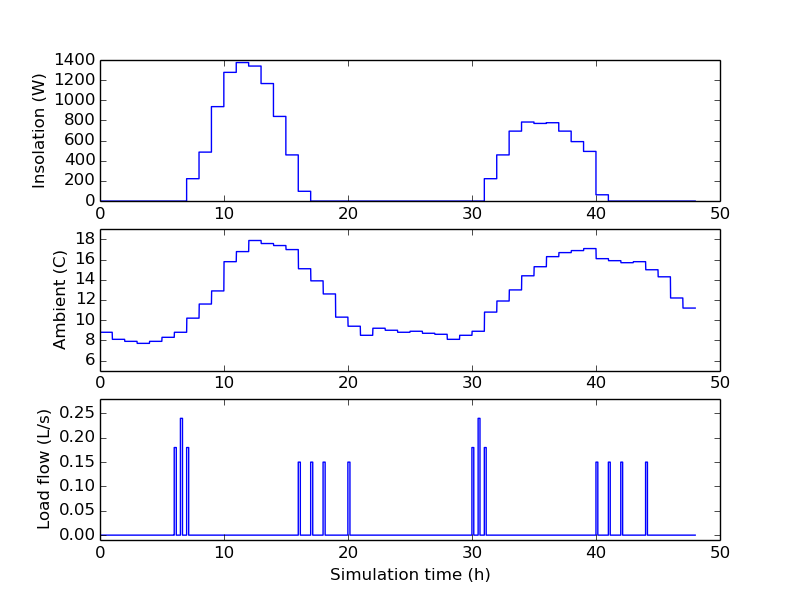
\includegraphics[width=10cm]{images/cer-data}
	\caption{Two days of simulated weather and load conditions}
	\label{fig:cer-data}
\end{figure}

\subsection{Metrics}

The controller's performance was quantified according to three metrics:

\begin{description}
	\item[Satisfaction]
		The user's satisfaction was measured by accumulating the total amounts of time when water was flowing to the user and was at least 50 degrees, and when water was flowing and was less than 50 degrees.
		This number was chosen based on guidelines for domestic water use from Sustainability Victoria~\cite{LSTS}.
	\item[Energy use]
		The total energy use of the controller is integrated across each experiment run.
		This provides an obvious way to compare the strategies of each controller based on how much power they consume to achieve the level of comfort measured by the first metric.
		Note that energy bill is assumed to be implicit in this metric, as this thesis does not take into account the effects of a varying energy price.
	\item[Solar contribution]
		The `solar contribution' refers to the amount of energy gained from sunlight relative to the total amount of energy put into the hot water tank.
		This is a relevant metric as it permits the examination of how effectively the solar resource was exploited.
		However, analysis is complicated by the relationship between solar fraction and total energy used by the controller.
		If one controller expends less control power, all else being equal, it will tend to have a higher solar contribution simply because the amount of energy gained from the sun is now greater in comparison.
		However, this metric does take into account the effect of a tank kept too-hot, which will result in the solar pump differential controller never choosing to let water enter the tank, thereby reducing solar contribution.
\end{description}

These metrics were evaluated each minute during the simulation.

\subsection{Experiment matrix}

Grid of variables that were used for each experiment.
Be sure to cover properties like handling an inaccurate prediction, and the effect of the PWM period.
